% generated by notebooks/thesis, do not edit by hand
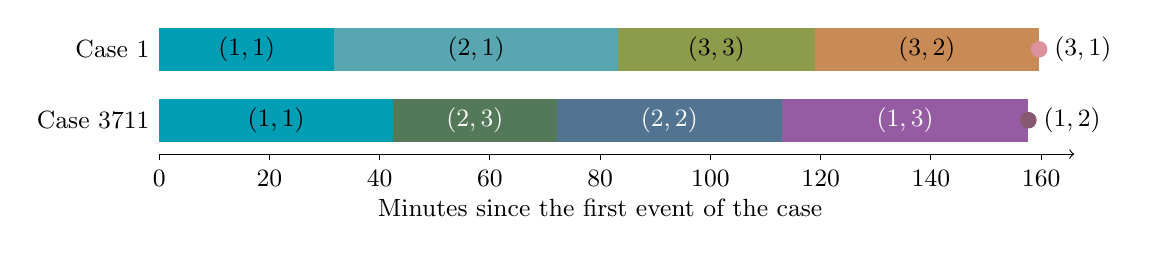
\begin{tikzpicture}[font=\small, x=0.07cm, y=1cm]
	\definecolor{trajectory0}{HTML}{009EB4}
	\definecolor{trajectory1}{HTML}{58A7B0}
	\definecolor{trajectory2}{HTML}{8D9C4A}
	\definecolor{trajectory3}{HTML}{C98B55}
	\definecolor{trajectory4}{HTML}{DB929C}
	\definecolor{trajectory5}{HTML}{547959}
	\definecolor{trajectory6}{HTML}{527491}
	\definecolor{trajectory7}{HTML}{955CA3}
	\definecolor{trajectory8}{HTML}{855A6E}
	\node[left] at (0, 0.28) {Case 1};
	\fill[trajectory0] (0.00, -0.00) rectangle (31.75, 0.55);
	\node[text=black] at (15.88, 0.28) {$(1, 1)$};
	\fill[trajectory1] (31.75, -0.00) rectangle (83.23, 0.55);
	\node[text=black] at (57.49, 0.28) {$(2, 1)$};
	\fill[trajectory2] (83.23, -0.00) rectangle (118.92, 0.55);
	\node[text=black] at (101.08, 0.28) {$(3, 3)$};
	\fill[trajectory3] (118.92, -0.00) rectangle (159.63, 0.55);
	\node[text=black] at (139.28, 0.28) {$(3, 2)$};
	\fill[trajectory4] (159.63, 0.28) circle (3pt) node[right=2pt, text=black] {$(3, 1)$};
	\node[left] at (0, -0.62) {Case 3711};
	\fill[trajectory0] (0.00, -0.90) rectangle (42.42, -0.35);
	\node[text=black] at (21.21, -0.62) {$(1, 1)$};
	\fill[trajectory5] (42.42, -0.90) rectangle (72.13, -0.35);
	\node[text=white] at (57.28, -0.62) {$(2, 3)$};
	\fill[trajectory6] (72.13, -0.90) rectangle (112.95, -0.35);
	\node[text=white] at (92.54, -0.62) {$(2, 2)$};
	\fill[trajectory7] (112.95, -0.90) rectangle (157.68, -0.35);
	\node[text=white] at (135.32, -0.62) {$(1, 3)$};
	\fill[trajectory8] (157.68, -0.62) circle (3pt) node[right=2pt, text=black] {$(1, 2)$};
	\draw[->] (0, -1.05) -- (166.00, -1.05);
	\draw (0, -1.05) -- (0, -1.13) node[below] {0};
	\draw (20, -1.05) -- (20, -1.13) node[below] {20};
	\draw (40, -1.05) -- (40, -1.13) node[below] {40};
	\draw (60, -1.05) -- (60, -1.13) node[below] {60};
	\draw (80, -1.05) -- (80, -1.13) node[below] {80};
	\draw (100, -1.05) -- (100, -1.13) node[below] {100};
	\draw (120, -1.05) -- (120, -1.13) node[below] {120};
	\draw (140, -1.05) -- (140, -1.13) node[below] {140};
	\draw (160, -1.05) -- (160, -1.13) node[below] {160};
	\node[below=0.45cm] at (80.0, -1.05) {Minutes since the first event of the case};
\end{tikzpicture}
